
\documentclass[conference]{IEEEtran}

% Paquetes

\usepackage[spanish]{babel}
 \usepackage{comment}
\usepackage{cite}
\usepackage{amsmath,amssymb,amsfonts}
\usepackage{algorithmic}
\usepackage{graphicx}
\usepackage{textcomp}
\usepackage{xcolor}
\def\BibTeX{{\rm B\kern-.05em{\sc i\kern-.025em b}\kern-.08em
    T\kern-.1667em\lower.7ex\hbox{E}\kern-.125emX}}

% Inicio del Documento

\begin{document}

\title{LABORATORIO N°7= DISEÑO ELECTRÓNICA I
}
\author{\IEEEauthorblockN{Brayan Andreys Gonzalez Perez }
\IEEEauthorblockA{1161828 \\
brayanandreysgope@ufps.edu.co}
\and
\IEEEauthorblockN{Juan David Olarte Pabon}
\IEEEauthorblockA{1162074 \\
juandavidolpa@ufps.edu.co}
\and
\IEEEauthorblockN{Yimar Andres Serna Silva}
\IEEEauthorblockA{1091762 \\
Yimarandressesi@ufps.edu.co}
}


\maketitle

\selectlanguage{english}
\setlocalecaption{english}{abstract}{Abstract} 
\begin{abstract}
This laboratory involved the design and analysis of a multistage voltage amplifier with a beta-independent stabilized Q-point, achieving a voltage gain of 25 using a 50mV sinusoidal signal at a frequency of 1kHz..\\
\end{abstract}
\renewcommand\IEEEkeywordsname{Keywords}
\begin{IEEEkeywords}
 Small-signal, Multistage, Amplifier.\\
\end{IEEEkeywords}

\selectlanguage{spanish}

\begin{abstract}
El presente laboratorio se realizo un diseño con analisis de pequeña señal con punto de Q estabilizado independiente de  beta multi etapa con una ganancia de voltaje de 25 con una señal de 50mv senoidal con frecuencia de 1khz .\\
\end{abstract}

\renewcommand\IEEEkeywordsname{Palabras Clave}
\begin{IEEEkeywords}
Pequeña señal, Multietapas, Amplificador.
\end{IEEEkeywords}


\section{Introducción}
Este ejercicio de laboratorio involucra el diseño y análisis de un amplificador de voltaje multietapa con un punto Q estabilizado independiente de beta. El objetivo de este ejercicio es brindar a los estudiantes la oportunidad de aplicar los conocimientos teóricos y criterios básicos adquiridos en los cursos de Electrónica I. Los estudiantes tendrán la oportunidad de desarrollar libremente su iniciativa y estudiar soluciones alternativas, diseñar y ensamblar completamente sistemas electrónicos (prototipos) que satisfagan las necesidades correspondientes.

\section{Objetivos}

\subsection{Objetivo General}

Diseñar y analizar un amplificador de voltaje multietapa con un punto Q estabilizado independiente de beta que cumpla con los requerimientos establecidos 

\subsection{Objetivos específicos}

Diseñar y evaluar amplificadores multietapa discretos e integrados empleando las diferentes técnicas de variación de la ganancia. \\

Integrar los conocimientos adquiridos en las diferentes asignaturas teóricas y prácticas vistas durante la carrera, en el diseño y desarrollo de proyectos.

\section{Desarrollo del Laboratorio}

El desarrollo de este laboratorio se efectúa en dos partes:\\
\begin{enumerate}
    \item El diseño del circuito amplificador conforme a las especificaciones requeridas, incluyendo el proceso matemático.
    \item La simulación de dicho circuito usando herramientas virtuales.
\end{enumerate}

\subsection{Diseño}
El diseño planteado para el multietapas consta de 3 etapas, siendo estas dos inversores para la ganancia y un seguidor para rectificar cualquier interferencia que se pueda producir.\\

\includegraphics[width=8.5cm]{imagenes/diseño_planteado.png}
\caption{Diseño propuesto. Las resistencias de $1\Omega$ representan valores desconocidos}

\subsubsection{ETAPA III: Emisor-Seguidor}


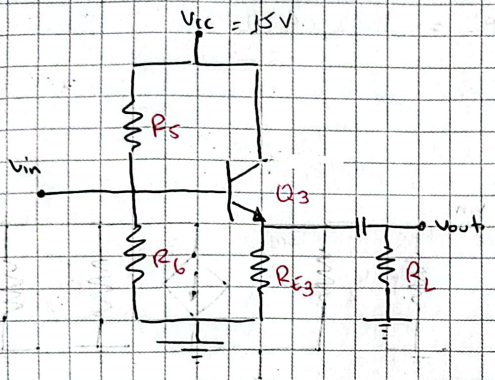
\includegraphics[width=4cm]{imagenes/etapa3.PNG}
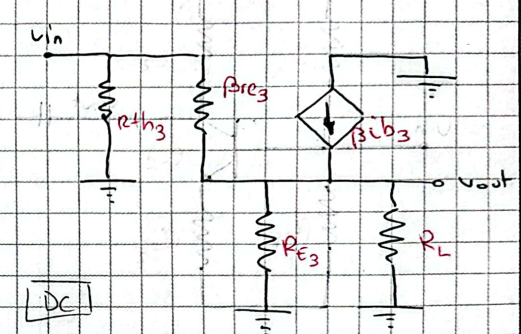
\includegraphics[width=4cm]{imagenes/etapa3.1.PNG}
\begin{center}
De acuerdo con las características establecidas en la hoja de datos del transistor \cite{Q2N2222A}, establecemos un $\beta$ de $240$:

\[\beta = 240\]

Se establece un voltaje de emisor-colector de $7.5V$ para que el transistor se encuentre en la región activa.
\[ 
R_{L} = 1k\Omega = R_{E3}; V_{CE} = 7.5v\]
\[I_{CQ} 0 \frac{V_{CC}-V_{CE}}{R_{E}}=\frac{7.5v}{1k\Omega} = 7.5mA \]
\[I_{sat}= \frac{15v}{1k\Omega} = 15mA \]

Usando los criterios de diseño para un transistor por polarización de divisor de voltaje de \cite{neamen2009microelectronics}:

\[R_{B3} = 0.1(\beta +1)=24.1k\Omega\]
\[\beta r_{e} = \frac{\beta V_{T}}{I_{CQ}}=800\Omega \]
\[V_{bb} = V_{BE}+ I_{CQ}((\frac{R_{B3}}{\beta})+R_{E}) \]
\[V_{bb} = 0.7v + 8.25v \]
\[V_{bb}= 8,95v \]
\[R_{6} = \frac{R_{B}}{1-\frac{V_{bb}}{V_{cc}}} = \frac{24100\Omega}{1-\frac{8,95v}{15v}} \]
\[R_{6} = 59794k\Omega \approx  60,4k\Omega \]
\[R_{5} =  \frac{R_{B}V_{CC}}{V_{BB}} \approx 40.2k\Omega\]

Hallamos la ganancia de la etapa haciendo un análisis en pequeña señal:

\[V_{out} = (R_{2}||R_{E2})(\beta +1)(ib_{3}) \]
\[I_{b3}= \frac{V_{i}}{(\beta r_{e3})+(\beta + 1)(R_{E} || R_{2})} \]
\[V_{out} = (v_{1})(\frac{(R_{L}||R_{E2})*(\beta+1)}{\beta r_{e3}+(\beta + 1)(R_{E}||R_{L})})\]
\[A_{V3} = \frac{500\Omega 241}{800\Omega + (241,500\Omega)}\]
\[A_{V3}=0.993\]

Y final mente hallamos la impedancia de entrada para la etapa 3 de la misma forma:

\[Z_{in3}=(\beta r_{e3} + (\beta + 1) (R_{1} || R_{2})|| R_{th})\]
\[Z_{in3}=20105,43 \Omega\]
\end{center}

\subsubsection{ETAPA II: Inversor}


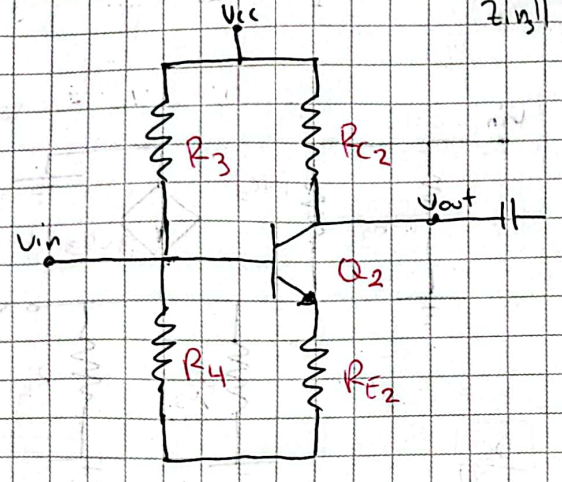
\includegraphics[width=4.5cm]{imagenes/etapa2.PNG}
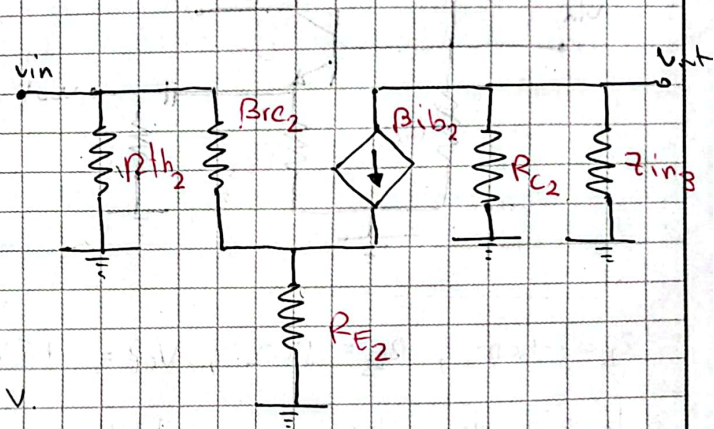
\includegraphics[width=4cm]{imagenes/etapa2.1.PNG}

\begin{center}

Se plantea una ganancia de -2.55 en esta etapa para compensar cualquier perdida de voltaje debido a la variación de las resistencias, ya que se debe obtener una ganancia de mínimo 25 al final. Del mismo modo, para el correcto funcionamiento de la etapa, $R_{C2}<<Z{in3}$, por tanto se plantea una resistencia $R_{C2}$ de $1.8k\Omega$

\[\beta = 240 ; A_{V2}=-2.55 ; Z_{in3}=20105,43 \Omega ; R_{c2}=1.8k \Omega\]
\[Z_{in}|| R_{e2} = 1652,09 \Omega\]

La impedancia de entrada de la siguiente etapa puede tratarse como una carga en esta etapa, por ello poedmos plantear que:

\[R_{L}= Z_{in3}=21915,68 \Omega; V_{CE}=7,5v\]

Mediante un análisis en pequeña señal del circuito hallamos la expresión para la ganancia del inversor:

\[V_{out}=-\beta b_{2} (R_{c2} || Z_{in3})\]
\[i_{b2}= \frac{V_{in}}{\beta r_{e2}+(\beta +1)R_{E2}}\]
\[V_{out}=-(\frac{\beta (R_{c2} || Z_{in3}) V_{i1}}{\beta r_{e2}+(\beta+1)R_{E2}})\]
\[A_{V2} =-(\frac{\beta(R_{c2}||Z_{in3})}{\beta r_{e2}+(\beta +1)R_{E2}})\]

Ahora, reemplazamos $\beta r_{e3}$ en términos de $R_{C2}$ y $R_{E2}$:

\[\beta r_{e2}=\frac{\beta v_{T}}{I_{ca}} ; I_{CQ}= \frac{7,5v}{R_{c}+R_{E}}\]
\[\beta r_{e2}=(\frac{\frac{\beta V_{T}}{1}}{\frac{7,5v}{R_{c}+R_{E}}}) = \frac{\beta V_{T}(R_{c}+R_{E})}{7,5v}\]

Reemplazamos en la expresión de la ganancia:

\[-2,55= -(\frac{\beta(R_{c2}||Z_{in3})}{(\frac{\beta V_{T} (R_{c}+R_{E})}{7,5v})+(\beta+1)R_{E2}})\]
\[\frac{\beta V_{T} R_{c}}{7,5v}+ \frac{\beta V_{T} R_{E}}{7,5v}+ (\beta+1) R_{E2} = \frac{\beta(R_{c2}||Z_{in3})}{2,55}\]
\[R_{E} =[\frac{\beta V_{T}}{7,5v}+(\beta +1)]= \frac{\beta(R_{c2}||Z_{in3})}{2,55}- \frac{\beta V_{T}R_{c}}{7,5v}\]
\[R_{E}(241,8)= 156150.59\Omega - 1440\]
\[R_{E}=\frac{154710.59\Omega}{241,8}\]
\[R_{E} = 639.83\Omega\]

Usando los criterios de diseño para un transistor por polarización de divisor de voltaje de \cite{neamen2009microelectronics}:

\[R_{B2}= 0,1(\beta+1)R_{E}=15429.90\Omega\]
\[I_{CQ}=\frac{7,5v}{R_{C}+R_{E}}=3,074mA\]
\[V_{BB}=V_{BE}+I_{CQ}(\frac{R_{B2}}{\beta}+R_{E})\]
\[V_{BB}=0,7V+2,164V\]
\[V_{BB}=2,864V\]
\[R_{4}= \frac{R_{B}}{1-\frac{V_{BB}}{V_{CC}}} = 19071.75\Omega\]
\[R_{3} = \frac{R_{B} V_{cc}}{V_{BB}}= 80801.74\Omega\]

Finalmente obtenemos la impedancia de entrada haciendo análisis en pequeña señal:

\[\beta r_{e2}= \frac{\beta V_{T}}{I_{CQ}}=1962,71\Omega\]
\[Z_{in2}= R_{th}|| [\beta r_{e2}+(\beta+1)R_{2}]\]
\[Z_{in2}=15429.90\Omega || 156150.88\Omega\]
\[Z_{in2}=14042.32\Omega\]

\end{center}

\subsubsection{ETAPA I: Inversor}

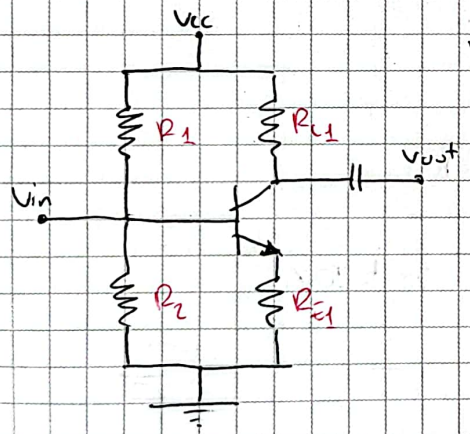
\includegraphics[width=4.5cm]{imagenes/etapa1.PNG}
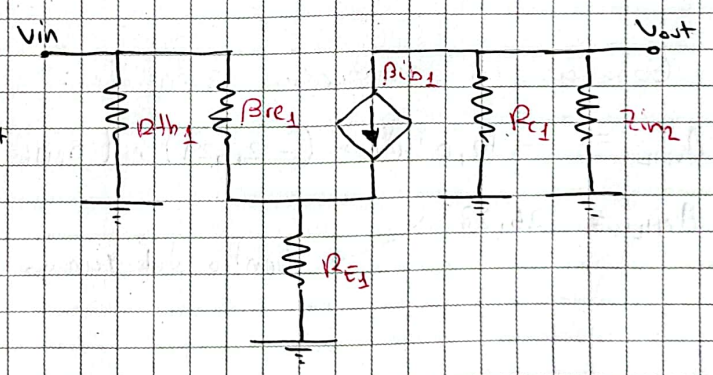
\includegraphics[width=4cm]{imagenes/etapa1.1.PNG}

\begin{center}

Se plantea una ganancia de -10.5 en esta etapa para compensar cualquier perdida de voltaje debido a la variación de las resistencias, ya que se debe obtener una ganancia de mínimo 25 al final. Del mismo modo, para el correcto funcionamiento de la etapa, $R_{C1}<<Z{in2}$, por tanto se plantea una resistencia $R_{C1}$ de $1.5k\Omega$

\[\beta =240; A_{V3}=-10.5 ; Z_{in2}=14042.32\Omega ; R_{c1}=1,5k\Omega \]
\[R_{C1}||Z_{in2}=1357,74\Omega\]

Usando la expresión hallada en la etapa anterior hallamos $R_{E1}$:

\[A_{V3}=-(\frac{\beta(R_{C1}||Z_{in2})}{\beta r_{e1}+(\beta +1)R_{E1}})\]
\[\beta r_{e2}= \frac{\beta V_{T}(R_{E}+R_{c})}{7,5v}\]
\[R_{E1}[\frac{\beta V_{T}}{7,5v}+(\beta+1)]=\frac{\beta(R_{c1}||Z_{in2})}{10.5}+ \frac{\beta V_{T} R_{c}}{7,5v}\]
\[R_{E1}(241,8)=30976.69\Omega - 1200\Omega\]
\[R_{E1}= \frac{29776.69\Omega}{241,8}=123.55\Omega\]

Usando los criterios de diseño para un transistor por polarización de divisor de voltaje de \cite{neamen2009microelectronics}:

\[R_{B1}=0,1(\beta +1) R_{E}=2967.92\Omega\]
\[I_{CQ}= \frac{7,5v}{R_{c}+R_{E}}=4,621mA\]
\[V_{BB}=V_{BE}+I_{CQ}(\frac{R_{B1}}{\beta}+R_{E})\]
\[V_{BB}=(0,7+0,626)v\]
\[V_{BB}=1,326v\]
\[R_{2}= \frac{R_{B}}{1- \frac{V_{bb}}{V_{cc}}}=3255.73\Omega\]
\[R_{1}=\frac{R_{B} V_{cc}}{V_{bb}}=33573.76\Omega\]

%Finalmente hallamos la impedancia de entrada para la etapa:

%\[\beta r_{e1}= \frac{\beta V_{T}}{I_{CQ}}=1303,78\Omega\]
\end{center}

\subsubsection{Análisis en pequeña señal}
Finalmente se realiza un análisis en pequeña señal del circuito en su totalidad:\\

Ganancia de voltaje con carga:\\
\[ A_{VT} = A_{V1} \times A_{V2} \times A_{V3} \]
\[ A_{VT} = -(\frac{\beta(R_{C1}||Z_{in2})}{\beta r_{e1}+(\beta +1)R_{E1}})\]
\[\times-(\frac{\beta(R_{C2}||Z_{in3})}{\beta r_{e2}+(\beta +1)R_{E2}}) \times (\frac{(R_{L}||R_{E3})*(\beta+1)}{\beta r_{e3}+(\beta + 1)(R_{E3}||R_{L})}) \]
\[ A_{VT} = -10.4991 \times -2.5392 \times 0.9934 \]
\[\boxed{ A_{VT} = 26.4837 }\]\\

Ganancia de voltaje sin carga:\\
\[ A_{VTNL} = A_{V1} \times A_{V2} \times A_{V3} \]
\[ A_{VTNL} = -(\frac{\beta(R_{C1}||Z_{in2})}{\beta r_{e1}+(\beta +1)R_{E1}})\]
\[\times-(\frac{\beta(R_{C2}||Z_{in3})}{\beta r_{e2}+(\beta +1)R_{E2}}) \times (\frac{(R_{E3})*(\beta+1)}{\beta r_{e3}+(\beta + 1)(R_{E3})}) \]
\[ A_{VT} = -10.4991 \times -2.5392 \times 0.9967 \]
\[ \boxed{ A_{VT} = 26.5714} \]\\ 

Ganancia de corriente con carga:\\
\[ A_{IT} = \frac{-\beta(R_{C2}||R_{5}||R_{6})}{(R_{C2}||R_{5}||R_{6})+(\beta r_{e3}+(\beta + 1)*((B+1)*R_{E3})||RL)}\]
\[ \times \frac{-\beta(R_{C1}||R_{3}||R_{4})}{(R_{C1}||R_{3}||R_{4})+(\beta r_{e2}+(\beta + 1)R_{E2})} \]
\[ \times \frac{(R_{1}||R_{2})}{(R_{1}||R_{2})+(\beta r_{e1}+(\beta + 1)R_{E1}))} \times (\beta + 1) \]
\[ A_{IT} =  (\beta + 1) \times -1.6578 \times -2.0828 \times 0.0874 \]
\[ \boxed{ A_{IT} = 72.7559} \]\\ 

Ganancia de corriente sin carga:\\
\[ A_{ITNL} = (\beta + 1) \times \frac{-\beta(R_{C2}||R_{5}||R_{6})}{(R_{C2}||R_{5}||R_{6})+(\beta r_{e3}+(\beta + 1)R_{E3})}\]
\[ \times \frac{-\beta(R_{C1}||R_{3}||R_{4})}{(R_{C1}||R_{3}||R_{4})+(\beta r_{e2}+(\beta + 1)R_{E2})} \]
\[ \times \frac{(R_{1}||R_{2})}{(R_{1}||R_{2})+(\beta r_{e1}+(\beta + 1)R_{E1}))} \]
\[ A_{ITNL} =  (\beta + 1) \times -1.6510 \times -2.0828 \times 0.0874 \]
\[ \boxed{ A_{ITNL} = 72.4583} \]\\ 

Impedancia de entrada con carga y sin carga:

\[ Z_{in} = (R_{1}||R_{2}) || (\beta r_{e1}+(\beta + 1)R_{E1}) \]
\[ \boxed{ Z_{in} = 2.708k\Omega} \]\\ 

Impedancia de salida con carga:

\[ Z_{o} = \frac{(R_{C2}||R_{5}||R_{6}) + \beta r_{e3}}{\beta + 1} || (R_{E3}||R_{L})\]
\[ \boxed{ Z_{in} = 10.0626\Omega} \]\\ 

Impedancia de salida sin carga:

\[ Z_{oNL} = \frac{(R_{C2}||R_{5}||R_{6}) + \beta r_{e3}}{\beta + 1} || (R_{E3})\]
\[ \boxed{ Z_{in} = 10.1649\Omega} \]\\ 
\begin{center}
\hspace{1cm}\\
\begin{tabular}{|c c c|}
		\hline
		Parámetro & CON RL & SIN RL \\ [1ex]
		\hline\hline
		$Av$ & $26.4837$ & $26.5714$ \\
        $Ai$ & $72.7559$ & $72.4583$ \\
        $Zo$ & $N/A$ & $10.1649\Omega$ \\
        $Zi$ & $N/A$ & $2.708k\Omega$ \\
		\hline
\end{tabular}
\hspace{1cm}\\    
\end{center}

%-------------------SIMULACIONES---------------------

\subsection{Simulación}
Se realizó la simulación tanto con los valores calculados como con valores comerciales de resistencias para ver la variación en el resultado.
\subsubsection{Usando los valores calculados}
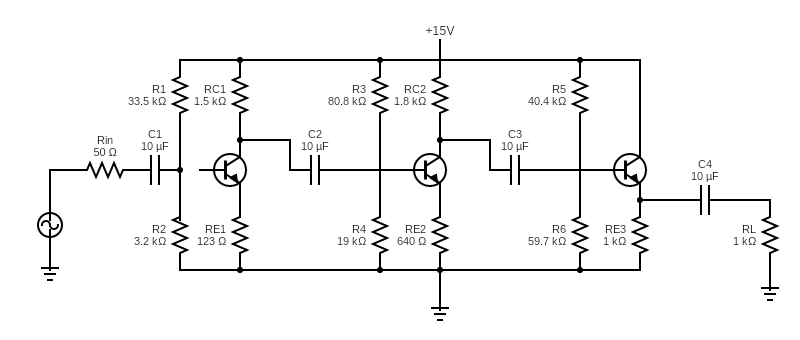
\includegraphics[width=9cm]{imagenes/valores_reales.png}
\begin{center}
\caption{Diseño propuesto con valores calculados}\\
\hspace{1cm}\\
\begin{tabular}{|c c c c|}
		\hline
		Resistencia & Valor & Resistencia & Valor \\ [1ex]
		\hline\hline
		$R1$ & $33.5k\Omega$ & $R2$ & $3.25k\Omega$\\
        $R3$ & $80.8k\Omega$ & $R4$ & $19k\Omega$\\
        $R5$ & $40.2k\Omega$ & $R6$ & $59.7k\Omega$\\
        $RE1$ & $123.15\Omega$ & $RC1$ & $1.5k\Omega$\\
        $RE2$ & $639.8\Omega$ & $RC2$ & $1.8k\Omega$\\
        $RE3$ & $1k\Omega$ & \hspace{1cm} & \hspace{1cm}\\
		\hline
\end{tabular}
\hspace{1cm}\\    
\end{center}
\begin{center}
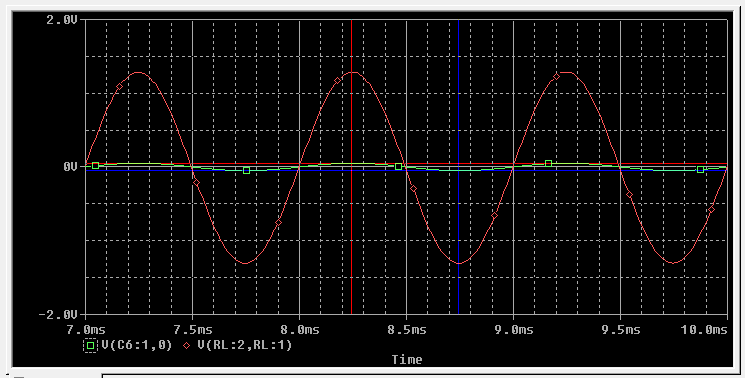
\includegraphics[width=9cm]{imagenes/simulacionrealgraph.png}
\caption{Gráficas de entrada y salida simuladas en OrCAD}\\
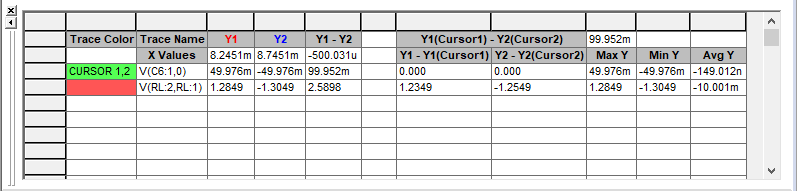
\includegraphics[width=9cm]{imagenes/simulacionrealdata.png}
\caption{Valores de los voltajes de entrada y salida}\\
\end{center}
\hspace{1cm}\\
\subsubsection{Usando valores de resistencias comerciales}
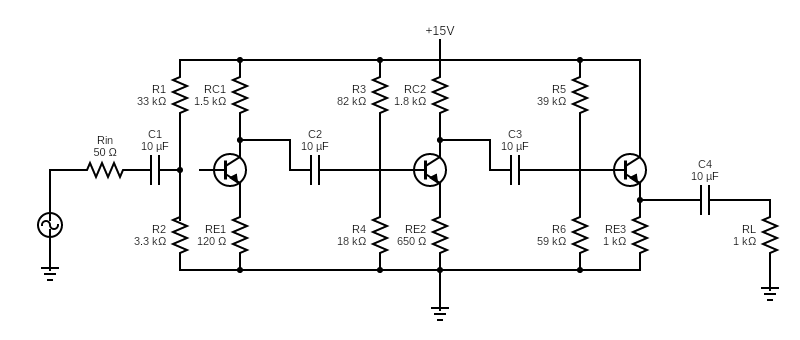
\includegraphics[width=9cm]{imagenes/valores_comerciales.png}
\begin{center}
\caption{Diseño propuesto con valores comerciales}\\
\hspace{1cm}\\
\begin{tabular}{|c c c c|}
		\hline
		Resistencia & Valor & Resistencia & Valor \\ [1ex]
		\hline\hline
		$R1$ & $33k\Omega$ & $R2$ & $3.3k\Omega$\\
        $R3$ & $82k\Omega$ & $R4$ & $18k\Omega$\\
        $R5$ & $39k\Omega$ & $R6$ & $59k\Omega$\\
        $RE1$ & $120\Omega$ & $RC1$ & $1.5k\Omega$\\
        $RE2$ & $650\Omega$ & $RC2$ & $1.8k\Omega$\\
        $RE3$ & $1k\Omega$ & \hspace{1cm} & \hspace{1cm}\\
		\hline
\end{tabular}
\hspace{1cm}\\
\end{center}
\begin{center}
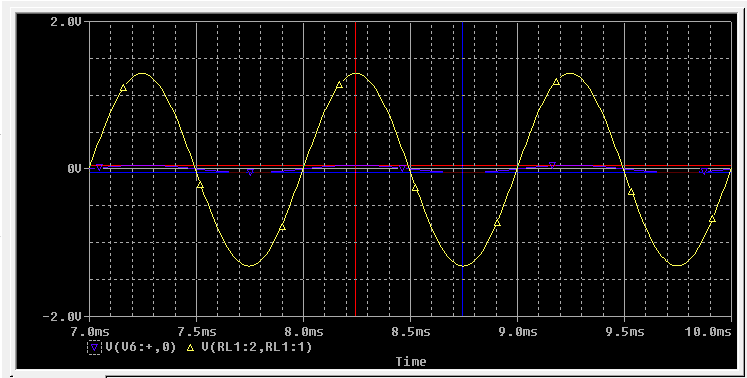
\includegraphics[width=9cm]{imagenes/simulacioncomergraph.png}
\caption{Gráficas de entrada y salida simuladas en OrCAD}\\
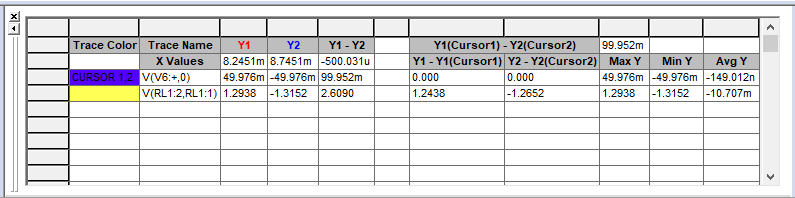
\includegraphics[width=9cm]{imagenes/simulacioncomerdata.png}
\caption{Valores de los voltajes de entrada y salida}\\
\end{center}
\section{Conclusiones}

\begin{itemize}
    \item La utilizacion de herramientas de simulacion permite validar el comportamiiento del circuito y evaluar su rendimiento del diseño en diferentes condiciones 

    \item El uso del emisor seguidor mejora la estabilidad y robustez del circuito frente a variaciones de carga lo que permite adaptabilidad a diferentes parametros de carga otorgados por su etapa anterior 

    \item se observa una leve variacion en la ganancia de voltaje total al utilizar valores comerciales de resistencias debido a que su comportamiento de la resistencia es dependiente de la tolerancia de trabajo efectivo que ella tenga de fabrica 
\end{itemize}



\begin{comment}
[1] Boylestad, R. L. (1999). Electronic devices and circuit theory (7a ed.). Prentice Hall. \\
no cambie eso
 [2] HAYT. (2018). Engineering Circuit Analysis. McGraw-Hill Education. \\

 [3] Newman, D. (2006). Circuit Analysis Exam File. Kaplan AEC Education.
\end{comment}
 
\bibliographystyle{IEEEtran}
\bibliography{Refs}



\end{document}

% Fin del documento